\documentclass[12pt]{article}
\usepackage{algorithm}
\usepackage{geometry}             
\usepackage{moreverb}   
\usepackage{fancyhdr}
\geometry{letterpaper}
\usepackage{algorithmic}             
\usepackage{algorithm}
\usepackage{array}     
\usepackage{hyperref}
\usepackage{graphicx}
\usepackage{subfigure}
\usepackage{fullpage}
\usepackage{amsmath, amssymb, amsthm}
\usepackage[framed,numbered,autolinebreaks,useliterate]{mcode}
\usepackage{mathabx}
\usepackage{float}

\newtheorem{theorem}{Theorem}
\newtheorem{corollary}{Corollary}
\newtheorem{proposition}{Proposition}
\newtheorem{lemma}{Lemma}
\newtheorem{definition}{Definition}
\newtheorem{remark}{Remark}
\newtheorem{notation}{Notation}

% my macros
\newcommand{\paren}[1]{\left({#1}\right)}
\newcommand{\bracket}[1]{\left[{#1}\right]}
\newcommand{\curly}[1]{\left\{{#1}\right\}}
\newcommand{\vecb}[1]{\mathbf{#1}}
\newcommand{\matb}[1]{\mathbf{#1}}
\newcommand{\V}[1]{\mathbf{#1}}
\newcommand{\m}[1]{\mathbf{#1}}
\newcommand{\inhomog}[1]{\widetilde{#1}}
\newcommand{\transpose}[1]{{#1}^\top}

\begin{document}

\title{CS 283 Final Project \\ Pipeline for Improving Accuracy of Hand Tracking with a Poorly Trained Haar Cascade Detector}
\date{Fall 2012}
\author{Kenny Yu, HUID: 30798260}
\maketitle

%%%%%%%%%%%%%%%%%%%%%%%%%%%%%%%%%%%%%%%%%%%%%%%%%%%%%
\section{Introduction}
What if you had the power of Microsoft's Kinect in your webcam? What if you could control applications simply with a swipe of your hand? Detecting and tracking hands typically requires a good detector, which requires large amounts of good data (usually at least 5000 images !!!CITE!!!) and a tremendous amount of computation time to train the classifier. In this paper, we trained our hand detector with only 250 images, generated from 10 positives and 100 negatives. Despite this poorly trained Haar cascade classifier, we provide a pipeline to improve accuracy during hand tracking, achieving comparable results to tracking with a well-trained hand detector. Using this pipeline, we create a sample application !!!CITE!!! in which the user can control Google Maps !!!CITE!!! by simply moving one's hand. See our source code in !!!CITE!!! for our pipeline and server to run this application.

\section{Methods}

\subsection{Training the Hand Detector}
To generate our hand detector, we took 10 pictures of our right hand using a webcam from a  Macbook Pro 2011 model, and we cropped the images to leave only our hand in the images. Our pictures consisted of our right hand with the palm facing forward and all fingers together. See Figure \ref{traininghands} for the the images we used as positives. We used the first 100 images from !!!!CITE!!!!! as negatives. We used OpenCV's \texttt{opencv\_createsamples} !!! CITE !!!!! utility to generate 250 90 $\times$ 50 pixel samples from this set of 10 positives and 100 negatives, resulting in images where our positive images have been warped by homographies and placed randomly into our negative images. We used OpenCV's \texttt{opencv\_haartraining} tool to train our Haar cascade classifier, setting our min hit rate to $0.999$, our max false alarm rate to $0.5$, and running 14 stages in our cascade. This took about a day to complete, and the resulting cascade is located in \texttt{cascades/hand\_front.xml}.

\noindent\begin{figure}[H]
\centering
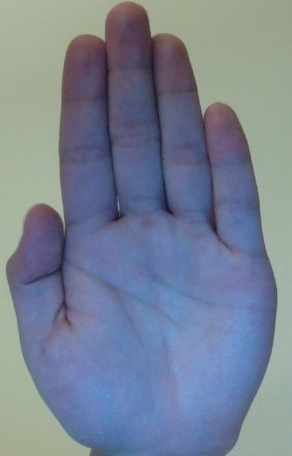
\includegraphics[width=50px, height=90px]{../data/positives/img0000.jpg}
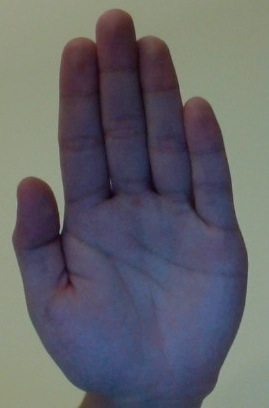
\includegraphics[width=50px, height=90px]{../data/positives/img0001.jpg}
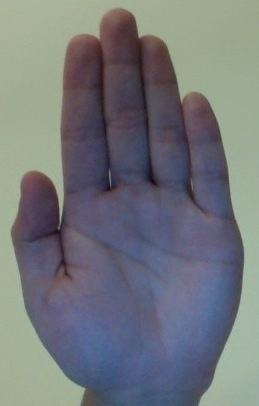
\includegraphics[width=50px, height=90px]{../data/positives/img0002.jpg}
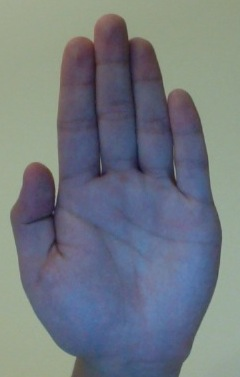
\includegraphics[width=50px, height=90px]{../data/positives/img0003.jpg}
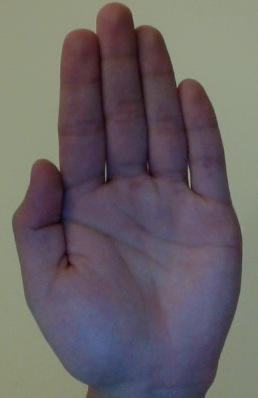
\includegraphics[width=50px, height=90px]{../data/positives/img0004.jpg} \\
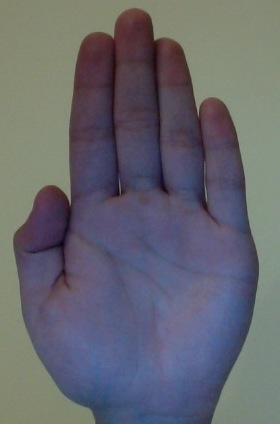
\includegraphics[width=50px, height=90px]{../data/positives/img0005.jpg}
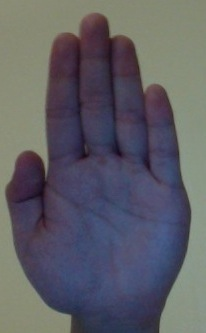
\includegraphics[width=50px, height=90px]{../data/positives/img0006.jpg}
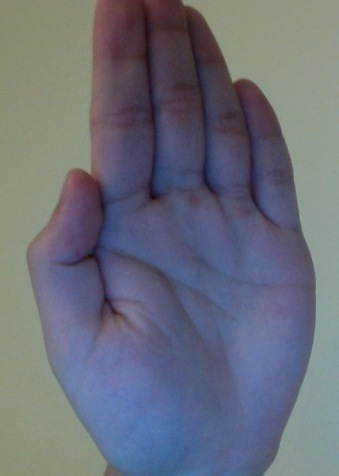
\includegraphics[width=50px, height=90px]{../data/positives/img0007.jpg}
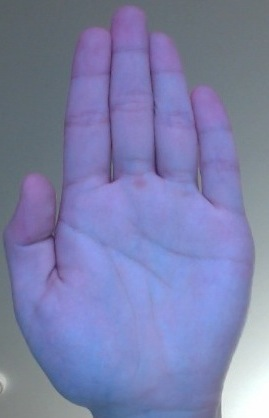
\includegraphics[width=50px, height=90px]{../data/positives/img0008.jpg}
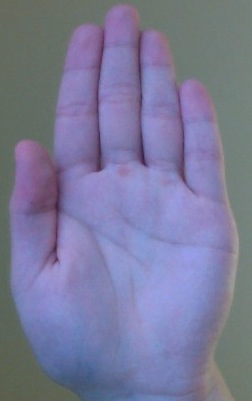
\includegraphics[width=50px, height=90px]{../data/positives/img0009.jpg}
\caption{The 10 positive images used to train our hand detector. We generated 250 samples from these, each of size 90 pixels high and 50 pixels wide.}
\label{traininghands}
\end{figure}

\subsection{Building the Pipeline}

See \texttt{detect.py} for the different components of our pipeline, and see \texttt{pipeline.py} for the various pipelines. For our pipeline, we used a frame size of 320 pixels wide and 240 pixels tall. We ran our detector without any preprocessing, and noted that we had many noisy detections, as shown in Figure \ref{1-original}. The yellow boxes indicate multiple possible detected hands, and the green one represents the largest one in the overall frame. We noted that our detector often mistook faces as hands, probably because of similar color tone. Using this heuristic, we decided to remove faces, and this generally gave us better results, as shown in \ref{2-noface}. We used OpenCV's frontal face detector in \texttt{cascades/haarcasacade\_frontalface\_alt.xml}, which works very well in practice.

Next, we noted that our detection was sensitive to noisy non-solid backgrounds. To account for this, we implemented background subtraction. To do this, we kept a history of the past $n$ frames, and we took the difference of the intensities of each pixel in the current frame and the oldest of the $n$ frames, and thresholded the difference. We found that setting our threshold to $20$ worked best, and we found that the number of frames $n = 20$ worked quite well. See Figure \ref{3-nobg} to see an example of the result of applying background subtraction. Background subtraction, however, had several issues. The dark patches left in the middle of the hand would sometimes prevent valid detections, and the randomly scattered dark patches also led to some false positive detections. 

To fix the latter issue, we used a simplified version of a Kalman Filter !!!! CITE !!!! to predict a bounding box window of where the hand would likely be in the next frame. We made the assumption that a hand typically moves in a smooth manner, and so using the velocity and current position of the hand will give us a pretty good prediction for where the hand will be in the next frame. 

We defined our state $\m{x_k}$ at step $k$ to be a 4-vector:
$$\m{x_k} = \transpose{(x, y, v_x, v_y)},$$
where $x,y$ is the current position (center) of the hand, and $v_x, v_y$ are the $x$ and $y$ components of the velocity of the hand. From this definition of our state, we naturally defined the next state (prediction) $\m{x_{k+1}}$ to be:
$$\m{x_{k+1}} = \transpose{(x + v_x, y + v_y, v_x, v_y)},$$
where we obtained the new $x,y$ components by adding the corresponding components in the velocity. Thus, our transition matrix $\m{A}$ satisfies the equation
$$\m{x_{k+1}} = \m{A} \m{x_k},$$
where
$$\m{A} = 
\begin{bmatrix}
1 & 0 & 1 & 0 \\
0 & 1 & 0 & 1 \\
0 & 0 & 1 & 0 \\
0 & 0 & 0 & 1
\end{bmatrix}.
$$
When we first attempted to use this Kalman filter, we had used error, process noise, and measurement noise covariance matrices, however, we discovered that reducing the Kalman filter to a simple Markov process improved runtime performance and greatly simplified the overall model. 

In our pipeline, we used our Kalman filter to predict a state $\m{x_{k+1}} = (x,y,v_x,v_y)$, where $(x,y)$ represents our prediction of the center of a $h \times w$ bounding box where we would probably detect our hand. In practice, we discovered that a $h = 180, w = 100$ worked best. Given this window, we applied our hand detector only within this window. See Figure \ref{4-kalman} for the result of this hand detection, and see the blue box in Figure \ref{5-optical} to see the Kalman prediction window relative to the original frame. 

We detected the corners within the detected hand, and then we used Lucas-Kanade !!! CITE !!! to compute the optical flow of these corners. We summed the overall displacements to obtain the overall velocity $(\hat{v_x}, \hat{{v_y}})$. To correct our estimate, we set our corrected state $\m{\hat{x_k}}$ to be:
$$\m{\hat{x_k}} = \transpose{(\hat{x}, \hat{y}, c\hat{v_x}, c\hat{v_y})},$$
where $(\hat{x},\hat{y})$ is the center of the detected hand, and $c$ is constant we chose to scale back the overall direction. If $c$ is too large, then our window will overshoot the position of the hand. If $c$ is too small, then our hand will move past the prediction window and will not be detected. In practice, we discovered that $c = 0.02$ works best. We then obtained our prediction $\m{x_{k+1}}$ for the next frame by using our corrected state $\m{\hat{x_k}}$:
$$\m{x_{k+1}} = \m{A} \m{\hat{x_k}}.$$
When there are no detected hands, we set our Kalman prediction to be the entire original frame. Our final pipeline is listed in Algorithm \ref{pipeline}.



\noindent\begin{figure}[H]
\centering
\subfigure[Our hand classifier had many noisy detections.]{
	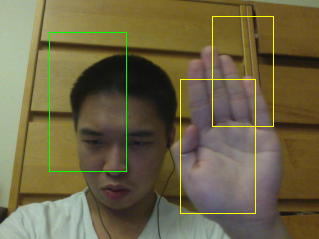
\includegraphics[width=220px, height=165px]{1-original.png}
	\label{1-original}
}
\subfigure[Face Removal]{
	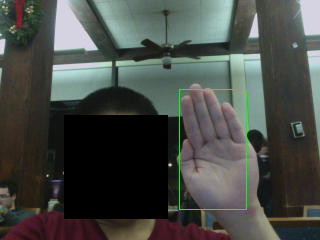
\includegraphics[width=220px, height=165px]{2-noface.png}
	\label{2-noface}
}
\subfigure[Background Subtraction]{
	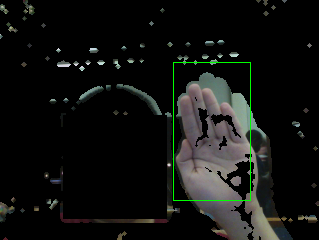
\includegraphics[width=220px, height=165px]{3-nobg.png}
	\label{3-nobg}
}
\subfigure[Kalman Prediction Window]{
	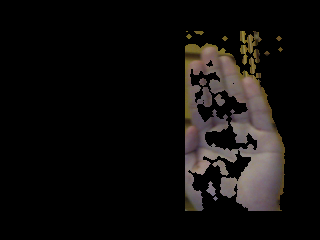
\includegraphics[width=220px, height=165px]{4-kalman.png}
	\label{4-kalman}
}
\subfigure[Final Detection and Optical Flow]{
	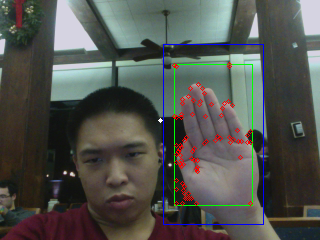
\includegraphics[width=220px, height=165px]{5-optical.png}
	\label{5-optical}
}
\caption{Our pipeline and hand detections at each stage. Green box - largest detected hand. Yellow boxes - other detections. Blue box - Kalman filter prediction. Red dots - corners.}
\label{all}
\end{figure}

\begin{algorithm}
\caption{Pipeline for Improving Accuracy of Hand Tracking with a Poorly Trained Hand Detector.}
\label{pipeline}

\noindent Given the current frame and the next frame:
\begin{enumerate}
\item {\bf Face Removal.} Apply OpenCV's frontal face detector and remove all detected faces.
\item {\bf Background Subtraction.} Eliminate the background through background subtraction.
\item {\bf Kalman Prediction.} Use our simplified Kalman filter to predict the likely bounding box of the hand in the current frame. If the previous frame had no detected hand, then our Kalman filter will estimate the entire frame as the bounding box.
\item {\bf Hand Detection.} Apply our hand detector within the bounding box (blue box) predicted by our Kalman Filter. If there are multiple detections (yellow boxes), take the first hand with the largest bounding box (green box)
\item {\bf Corner Detection.} If there are no detections, then output $(0,0)$ as our velocity. If there is a detection, compute the corners (red points) within the bounding box of our hand.
\item {\bf Optical Flow.} Use Lucas-Kanade to compute the optical flow of the detected corners, finding the corresponding points (if they exist) in the subsequent frame. Sum all the vector displacements (green vectors) to compute the overall velocity of the hand (white vector).
\item {\bf Kalman Update.} Update our Kalman Filter with the measured position and velocity of our detected hand, and repeat on the next frame.
\end{enumerate}
\end{algorithm}

\subsection{Building the Google Maps Application}

We used our pipeline to create a simple application in which the user can control Google Maps by moving one's hand. We follow the model proposed in !!!CITE!!! to create our application. We used Chrome's WebRTC ability to capture a video stream from a connected webcam. Using web sockets !!!CITE!!!, we send a constant stream of frames to our server that is running our pipeline. We used Tornado 2.4.1 !!!CITE!!! to run our server, and we used OpenCV 2.4.1 !!!CITE!!! to implement our pipeline. The server runs the pipeline and outputs the annotated frame and the overall computed direction of the hand, and the client then uses this information to update the map accordingly. A live running instance of the application can be publicly accessed at \url{http://goo.gl/pcNxG}. See Figure \ref{map} for a screenshot of the application in action. The green vectors represents the direction of the corners, and the white vector is the sum of the green vectors, representing the overall direction of the hand.

\noindent\begin{figure}[H]
\centering
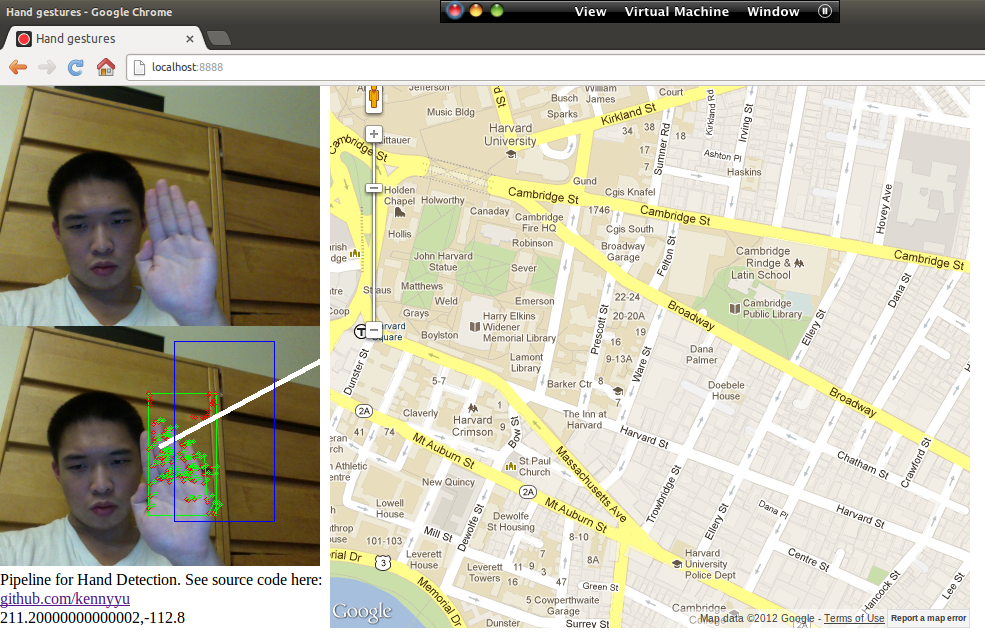
\includegraphics[scale=0.45]{map.png}
\caption{Screenshot of our Google Maps Application in action. The green vectors represents the direction of the corners, and the white vector is the sum of the green vectors, representing the overall direction of the hand.}
\label{map}
\end{figure}

\section{Results}

Background subtraction no good, too slow, better not to use it. 

\section{Conclusion}

\section{References}

\end{document}